% Wer Debian hat, kann LaTeX mit diesem Befehl installieren:
%  apt-get install  texlive texlive-lang-german texlive-latex-extra \
%  texlive-pictures texlive-science texlive-fonts-extra
% pdf generieren unter Linux:
%  pdflatex --output-directory /var/www/html/tmp/ serienmails.tex

% Diese Vorlage dient als Hilfestellung bei der Erstellung der schriftlichen
% Arbeit (die sogenannte Langfassung). Du bist nicht verpflichtet sie zu nutzen.
% Sie wurde zur Verf"ugung gestellt von Thomas@Wirsings.eu
%
% Die angef"uhrten Fragestellungen und Kommentare dienen nur als Anregung oder
% Checkliste, was bei einer Jugend forscht Arbeit beachtet werden sollte. Sie
% m"ussen nicht alle beantwortet werden. Weitere Hinweise findest Du im
% "Leitfaden zum Verfassen der schriftlichen Arbeit'' auf unserer Internetseite:
% www.jugend-forscht.de/teilnahme/ablauf/schriftliche-arbeit.html.
%
% Die Angaben zur Seitenanzahl dienen nur als grobe Orientierung, welchen Umfang
% die einzelnen Teile haben k"onnen.
%
% Du kannst Deinen Text einfach unter die Gliederungspunkte schreiben und daf"ur
% die Leitfragen und Kommentare l"oschen. Das Commando "\tbd" kann man nutzen um
% Teile zu markieren die noch nicht fertig sind.

\documentclass[12pt,twoside]{article}  % darf nicht kleiner sein (Vorgabe JuFo)
\pagestyle{headings}
\pagenumbering{Roman}
\usepackage[ngerman]{babel}
\usepackage[hidelinks]{hyperref}
\usepackage[a4paper]{geometry}
\usepackage{datetime}
\usepackage{graphicx}
\usepackage{color}
\usepackage[T1]{fontenc}
\usepackage[utf8]{inputenc}
\usepackage{charter}
\usepackage{tabularx}

\usepackage[official]{eurosym}
%\usepackage[hmargin=1in,vmargin=1in]{geometry}
\usepackage{listings}
% wegen deutschen Umlauten
% \usepackage[ansinew]{inputenc}

\definecolor{codegreen}{rgb}{0,0.6,0}
\definecolor{codegray}{rgb}{0.5,0.5,0.5}
\definecolor{codepurple}{rgb}{0.58,0,0.82}
\definecolor{backcolour}{rgb}{0.95,0.95,0.92}
 
\lstdefinestyle{mystyle}{
    backgroundcolor=\color{backcolour},   
    commentstyle=\color{codegreen},
    keywordstyle=\color{magenta},
    numberstyle=\tiny\color{codegray},
    stringstyle=\color{codepurple},
    basicstyle=\footnotesize,
    breakatwhitespace=false,         
    breaklines=true,                 
    captionpos=b,                    
    keepspaces=true,                 
    numbers=left,                    
    numbersep=5pt,                  
    showspaces=false,                
    showstringspaces=false,
    showtabs=false,                  
    tabsize=2
}
\lstset{style=mystyle}

\newcolumntype{C}[1]{>{\centering\arraybackslash}p{#1}}
\geometry{left=25mm,right=25mm, top=25mm, bottom=20mm}
  % R"ander bitte nicht kleiner (Vorgabe JuFo)
\setlength{\parindent}{0mm}

\newcommand{\tbd}[1]{\textcolor{red}{\large \bf tbd: #1}}

\begin{document}
  \title{Serienmails statt Papier}
  \setlength{\parskip}{0ex}
  \date{\today \ \currenttime \ MEZ}
  \maketitle
  \begin{center}
	  
\includegraphics[width=0.9\textwidth]{Titelbild.png}
	  % Quelle: https://pixabay.com/de/brief-email-mail-hand-schreiben-2794672/
  \end{center}

  \begin{center}
	     \vspace{2.385pt}\nointerlineskip\rule{\textwidth}{0.4pt}\\
	  In meinem Projekt 
%\glqq Serienmails\grqq{} 
          geht es darum m"oglichst viele Serienbriefe durch Serienmails zu ersetzen und dadurch umweltsch"adliches Papier zu sparen. 
          Daf"ur habe ich eine Webanwendung programmiert die beide Aspekte kombiniert. Diese sendet eine Einladungsmail f"ur Vereinsveranstaltungen, bei der
	  für jeden Benutzer, ein anderer Link generiert und am Ende der Email anf"ugt wird. Durch das Anklicken dieses Links durch den Empf"anger 
          wird dies in die MySQL Datenbank übertragen. Anhand dieser Datenbank sieht der Schriftf"uhrer auf einen Blick, wer die Mail noch nicht gelesen 
	  hat. Nur f"ur diese Leute wird ein Papierbrief generiert. Somit kann Papier gespart werden. Dies wiederum schont die Umwelt und spart 
	  Kosten. Getestet wird diese Software bei der 
	  \glqq Concordia Westhausen\grqq. Selbstverst"andlich kann das Vereinsmitglied auf der Weboberfl"ache auch angeben, mit wievielen Personen er zu diesem Event kommt.\\
	     \vspace{2.385pt}\nointerlineskip\rule{\textwidth}{0.4pt}\\
  \end{center} 


  \vfill
  \begin{center}
  \begin{tabular}{C{0.5\textwidth}C{0.5\textwidth}}
    \textbf{Luca Lutz} \\
    \textbf{M"uhlstra"se 7/1} \\
    \textbf{73463 Westhausen} \\
    \textbf{lucas.handy.1234@gmail.com} \\
  \end{tabular}
  \end{center}
  \vfill

  \hrulefill

  \parbox{\textwidth}{\centering \bf Jugend-Forscht 2019 ---
    Regionalwettbewerb Oberkochen --- \\
    Fachbereich Informatik}
  \thispagestyle{empty}
  \newpage

  \tableofcontents
  \listoffigures
  \listoftables
  %\listoftables
  \setlength{\parskip}{1ex}
  \cleardoublepage
  \pagenumbering{arabic}

  % ab hier max 15 Seiten % (Vorgabe JuFo)

  \section{Einleitung und Ziel} % 1 bis 2 Seiten
    \subsection{Problem}
    Auf dieses Thema bin ich bei der Concordia Westhausen, bei dem meine Mutter Mitglied ist, aufmerksam geworden. 
    Das Problem ist, dass bei Vereinen wichtige Briefe und Einladungen per Papier verschickt werden. Der Grund hierf"ur ist, 
    dass Papierbriefe zuverl"assiger als Emails gelten. Die Masse an Papier, die dabei entsteht, kommt einem zwar erst einmal 
    wenig vor. Man muss aber bedenken, dass es nicht nur eine Versammlung pro Jahr gibt, sondern auch noch, au"ser der 
    Hauptversammlung, zum Beispiel das Sommerfest und eine Winterwanderung. Zudem hat ein Verein schnell einmal >500 Mitglieder.
    Pro Event w"urden die Einladungen in diesem Fall bei Recyclingpapier \textbf{2,8kg} Holz, \textbf{20g} CO2 und \textbf{51,1 Liter} Wasser unn"otig ver(sch)wenden (laut Papierrechner \cite{Papiergewicht}). Doch auch bei einer Mail fallen 10g CO2 an. Bei Neupapier werden noch viel mehr Ressourcen verschwendet. 
    
    Viele Leute haben heutzutage allerdings Zugriff auf das Internet und E-Mail. Das hört sich ja eigentlich 
    nach der Lösung an, dachte ich mir. Allerdings weiß man nie, wer kommt und wie
    viele Leute sie mitbringen. Vor allem kann nie sichergestellt werden, ob der Empf"anger die
    E-Mail gelesen hat oder dieser schreibt eine Antwort per E-mail was viel Zeit in Anspruch 
    nimmt, weil es manuell ausgewertet werden muss.

    \subsection{Idee}
    Meine Idee was es deshalb eine Website zu programmieren, von der aus man eine Serienmail 
    verschicken kann. Das Programm f"ugt darunter einen Link ein, der bei Bet"atigung in eine
    Datenbank einträgt wer mit wie vielen Personen kommt. Zudem sollte es eine Option
    geben mit der man eintragen kann, dass man nicht kommet. Dadurch l"asst sich
    der unnötige Papierverbrauch abschaffen oder vermindern. Zudem weiß der Veranstalter
    gleich wie viele Leute teilnehmen.

    \subsection{Aktueller Stand}
    Event Organisationssoftware wie z. B. Doodle \cite{Doodle} oder LamaPoll \cite{LamaPool} gibt es. Allerdings werden dort  
    die Einladungen per E-Mail versendet. Leider haben diese aber
    das Defizit, dass sie bei wichtigen Veranstaltungen untauglich sind, da nur die Personen registriert 
    werden die das Internet nutzen. Dadurch werden dort sehr oft Einladungen per
    Papier verschickt. Dies ist eigentlich unn"otig. Mein System k"ummert sich auch darum, dass die Leute die kein Internet 
    nutzen oder die Mail noch nicht gelesen haben, einen Brief geschickt bekommen. 
    Von den Teilnehmern haben wir eine Best"atigung, dass die Mail gelesen wurde. Zudem wird "uber die Datenbank erfasst und 
    ausgewertet, wer mit wie vielen Personen teilnimmt oder an der Teilnahme verhindert ist. Somit hilft mein Programm der Umwelt und dem Schriftf"uhrer oder Vorstand. 


  \section{Vorgehensweise und Methode} % 2-6 Seiten 
  Eigentlich war mein Plan alles in PHP 
  \cite{php} 
  aufzubauen, da ich wusste, dass PHP E-Mails versenden kann. 
  Als ich sp"ater noch eine MySQL Datenbank erstellt habe, konnte ich auch diese in PHP einbinden. Mails versende 
  ich aber mit Postfix \cite{postfix} über die Linux Shell, weil ich dies als die Bessere Lösung ansehe. Darum habe ich ein Shellscript geschrieben, dass 
  Postfix ansteuert, allerdings verwende ich hier \glqq mailutils\grqq{} als Brücke um Postfix anzusteuern. 
 
  In diesem Script habe ich eine For Schleife, die sich aus der MySQL 
  Datenbank die E-Mailadressen aller Benutzer holt und an diese Personen eine E-Mail, mit dem von PHP importierten 
  Text und jeweils einem spezifischen Link darunter, sendet.
 
  Soweit zur Idee. In der Praxis wollte ich allerdings als Erstes 
  mit der Webgui anfangen. Dies habe ich auch getan. Es stellte sich jedoch schnell heraus, dass ich 
  sinnvollerweise bei der Datenbank und den Mails anfangen sollte. Erst ganz zum Schluss, wenn bereits 
  die gesamte Datenbankstruktur umgesetzt ist, macht es Sinn die Webgui zusammenzustellen. Dies ging viel 
  besser. Daraus lernte ich immer bei den \glqq unteren\grqq{} Softwareschichten 
  \cite{softwareschichten} 
  anzufangen. Dies nennt sich 
  \glqq bottum up\grqq{}. Die gegens"atzliche Vorgehensweise nennt sich \glqq top down\grqq{} und ist ein typischer Anf"angerfehler der zu Problemen f"uhrt.
  
  %\cite{Papierbrief}
  Der eigentliche Vorteil meines Programmes ist es, dass es auch Papierbriefe exportieren kann. Somit sind die Benutzer ohne Internet nicht ausgeschlossen. 
  Dies habe ich in einer PHP Seite umgesetzt, die ein Linux Skript aufruft. Die f"ur die einzelnen Benutzer spezifisch generierten Papierbriefe werden als 
  plain Text exportiert und zum Download als Zip-Datei angeboten.
 
  \subsection{Datenschutz/Datensicherheit}
Da die Datensicherheit noch wichtiger ist als Papier zu sparen, habe ich umfassend "uber die Sicherheit nachgedacht und mir sind folgende Risiken aufgefallen:
          %Problem           L"osung
          \begin{itemize}
	  \item Persönliche Daten von den Mitgliedern müssen vor Diebstahl geschützt sein: Auf die Daten hat nur der Schriftf"uhrer Zugriff \\
          \item Wiedereinspielen der Links: Die Links sind per Zufallszahl nur einmal verwendbar \\
          \item Man-in-the-Middle-Angriff:  Wird per TLS "ubertragen und ist somit nicht manipulierbar \\
          \item Mails f"alschen:  Nein, da nur die Software Zugriff auf den Mailserver hat \\
	  \item Die Datenbank vor Fremdzugriff schützen: Die Datenbank ist nur per Webgui erreichbar, der WWW User hat nur eingeschr"ankte Rechte \\
	  %\item Wichtige Daten f"ur alle sichtbar: Adminschutz mit MD5 gehashtem Password \\
	  \item Adminpasswort austestbar: Nein, da MD5 gehasht \\
	  \item Hash kann man cracken: Ja, aber braucht sehr lange und ist sehr schwer Dank MD5 \\
          \end{itemize}

%\begin{itemize}
%\item Wiedereinspielen der Links
%\item Man-in-the-Middle-Angriff 
%\item Mails f"altschen
%\item Die MySQL-Server vor Admin schützen
%\item Persöliche Daten von den Mitgliedern müssen geschützt sein
%\item Wichtige Daten f"ur alle sichtbar.
%\item Adminpasswort auslesbar.
%\item Hash kann man knacken.
%\end{itemize}

%\item Das login ist sehr sicher da das Password mit einem MD5-Hash und somit f"ur fremde unlesbar abgesichert wird.
%\item MD5 Link nuestes Standart
  
  \subsection{MySQL}
  In MySQL 
  \cite{mysql} 
  erstellte ich einen gesicherten User und eine Datenbank mit dem Namen \glqq Serienmails\grqq, die die Tabellen \glqq events \grqq, 
  \glqq users\grqq{} und \glqq einladungen\grqq{} enth"alt. In der Tabelle \glqq events\grqq{} stehen die Veranstaltungen, die Pfade 
  zu den Mailinhalten, sowie die Pfade zu den Anh"angen. Die Tabelle \glqq users\grqq{} enth"alt von jedem 
  User die E-mail und den Benutzernamen. Die Tabelle \glqq einladungen\grqq{} enth"alt von jedem Benutzer jedes Event 
  und den Status (kommt nicht, kommt allein, kommt mit 1/2/3/4/5, mehreren Personen).
  \subsection{PHP}
  Im Folgenden das Beispiel von der \glqq offene Events\grqq{} Transaktion (Dies ist nur ein Beispiel, alle anderen 
  Transaktionen sind "ahnlich aufgebaut). Mein gesamtes Programm umfasst zum jetzigen Zeitpunkt \textbf{1713} Zeilen PHP und Linux Code.
  \lstinputlisting[language=php]{offen.php}
  %\lstinputlisting[language=php]{/var/www/html/webgui/offen.php}
  Hier das Ergebnis dieses Quellcodes:
\begin{center}
%\begin{figure}
  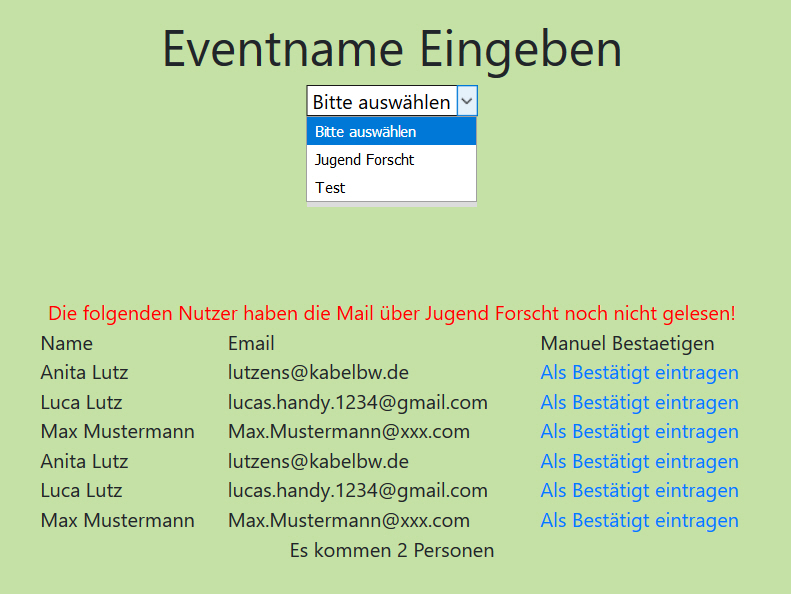
\includegraphics[width=0.5\textwidth]{code-ergebniss.jpg}
%\end{figure}
\end{center}
  Hier noch beispielhaft der MySQL Connector: 
  \lstinputlisting[language=php]{/var/www/html/webgui/connect.php}
  Die Abbildung stellt den MySQL Connector dar, der meine MySQL-Datenbank mit PHP verbindet. Er besteht im 
  Wesentlichen aus Variablen (Servername, Benutzername, Passwort und 
  Datenbanknamen). Darunter ist noch ein PHP Befehl der  
  eine Verbindung zu MySQL aufbaut. 
  PHP ist in meinem gesamten Projekt f"ur die Dynamik verantwortlich. Die 
  Websitestruktur ist in HTML geschrieben und anhand dem Beispiel \cite{bootstrapExample} in CSS 
  mit dem \glqq Bootstrap\grqq{} Framework gestylt. Den Datei-upload habe ich allerdings ohne Framework aber trotzdem in CSS programmiert, da ich dies dadurch freier gestalten konnte. (z.B. Drag\&Drop Men"u).
  
  \subsection{Linux}
  Beispiel Linux Programmzeilen:  
  \lstinputlisting{/home/luca/serienmails/webgui/mails_for.sh}
  Hier werden an alle Vereinsmitglieder Mails versendet. Dies geschieht "uber den Linuxdienst Postfix.
  %\subsubsection{Postfix}
  %\subsubsection{Apache}
  \subsection{Dokumentation}
  Ich habe gelernt alles zu dokumentieren da es dadurch reproduzierbar ist. Dies habe ich immer wieder in einem Life System getestet.
  Ich habe die gesamte Dokumentation in \textbf{Linux} und meine Langfassung in \textbf{Latex} geschrieben, so dass man es einfach mit \glqq./\grqq{} ausf"uhren 
  kann. Somit ist dies ebenfalls reproduzierbar. Zudem verwende ich Git, dass alles noch einmal 
  in der \glqq Bitbucket\grqq{} Cloud sichert, ca. 500 Zeilen Latex Code. \\
  Hier noch ein Bild um zu zeigen, wie ich in \textbf{Latex} diese Langfassung erstellt habe. 


  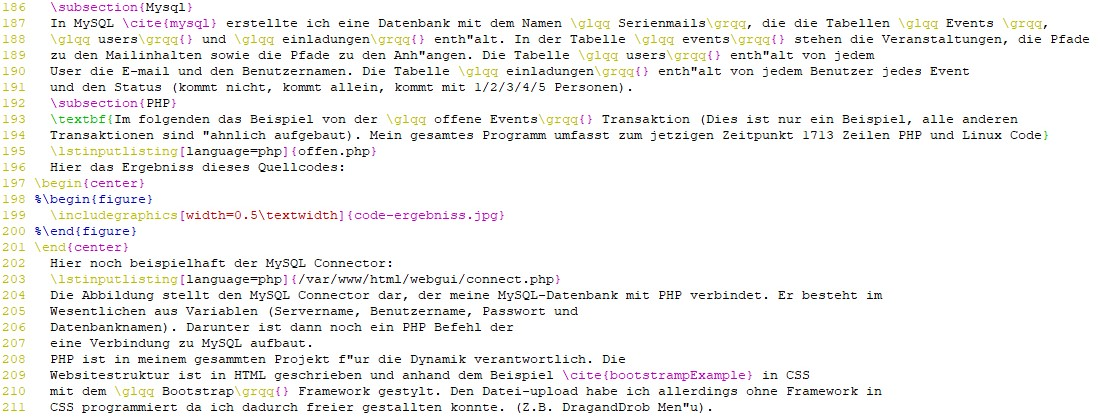
\includegraphics[width=1\textwidth]{beispiel_latex.jpg}
  \subsection{Zertifikat}
  Um bei den Mailprovidern, wie zum Beispiel gmail.com, gmx.net, outlook.de Vertrauen 
  zu gewinnen und um ein sicherer E-Mailabsender zu sein brauchte ich ein Zertifikat. Durch dieses Zertifikat wird meine Webgui 
  als sicher im Browser angezeigt. Das Zertifikat kann man sich entweder 
  selbst erzeugen z.B. mit OpenSSL (diesem wird aber nicht vertraut) oder man 
  l"asst sich eines von Letsencrypt \cite{letsencrypt} ausstellen. Dadurch bekommt man sogar ein 
  Wildcard Zertifikat, das bei professionellen Anbietern (in diesem Fall Symantec) 
  2499\euro{} kosten w"urde Abb. \ref{ZertProf}. Wie ich dieses Zertifikat kostenlos erstellt habe ist unter \url{papier.lucalutz.org/doku/}
  dokumentiert. 
  Wichtig ist hierbei zu sagen, dass sich meine Doku auf meine Domain 
  (\url{papier.lucalutz.org}) und meinen DNS Provider (\url{dynu.com}) bezieht. Um sich selbst ein Wildcard 
  Zertifikat auszustellen zu lassen, muss man diese Daten anpassen. F"ur ein normales Zertifikat reicht ein  
  Webserver wie Apache2 oder ein tempor"arer Webserver. Bei diesem werden die Daten in das 
  \glqq Document Web Root Directory\grqq{} des Webservers abgelegt. Da diese Zertifikate Abb. \ref{ZertLuca} aber nur 3 Monate halten, 
  muss man sie leider alle 3 Monate erneuern. Das Zertifikat kann man mit folgendem Code unter Linux anschauen: \lstinputlisting{openssl.sh}
  \begin{figure}
    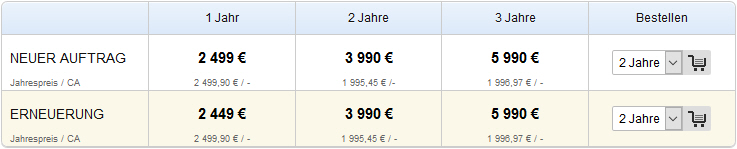
\includegraphics[width=0.7\textwidth]{zertifikat.jpg}
    \caption{Preise bei einem professionellen Hoster \label{ZertProf}}
  \end{figure} 
  \begin{figure}
    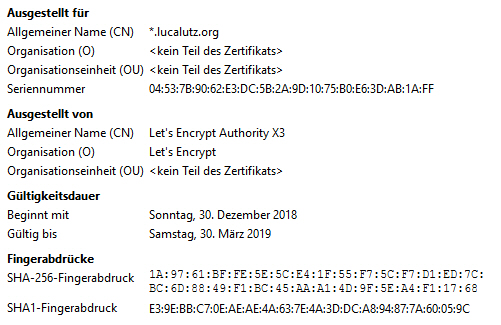
\includegraphics[width=0.5\textwidth]{ssl.jpg}
    \caption{Mein Zertifikat \label{ZertLuca}}
  \end{figure} 
  
    \subsection{Output}
Hier noch jeweils ein Beispiel von einer Mail Abb. \ref{MailEinladung} und einem Papierbrief: Abb. \ref{PaierbriefEinladung}\\
%Mail:
\begin{figure}
    \begin{verbatim}
    Betreff: Aktuelle Veranstaltung
    An: lutzens@kabelbw.de  

    Hallo Anita Lutz, 
    ich lade dich zu Jugend Forscht ein.

    Bitte mit diesem Link bestätigen:
    https://lucalutz.org/webgui/bestaetigung.php
    ?hash=0cf1b522bea677f69b6b0beab2e03f40&signup= 
    \end{verbatim}
    \caption{Einladung per Mail \label{MailEinladung}}
\end{figure}

%Papierbrief:
\begin{figure}
    \begin{verbatim}
    Germany, 89160 Dornstadt
    Mozartstraße 5


    Hallo Peter Wirsing,
    ich lade dich zu Jugend Forscht ein.
    \end{verbatim}
    \caption{Einladung per Papierbrief \label{PaierbriefEinladung}}
\end{figure}

  \section{Ergebnisse} % 2-5 Seiten
    Am Ende meiner Arbeit habe
    ich eine Software in PHP und Linux-Bash geschrieben, die genau meinen Anforderungen entspricht. 
    So kann diese eine Tabelle mit den Benutzern verwalten (Anlegen und L"oschen), eine E-Mail mit einem 
    Link versehen, der für jeden Benutzer unterschiedlich ist (Zusammensetzung: Username + Zufallszahl 
    + Eventname). Diese Daten werden zu einem Hash zusammengef"ugt und sind Dank der Zufallszahl nicht 
    vorhersehbar. Somit ist eine hohe Sicherheit gewährleistet. Die Daten werden ausgewertet und dem 
    Schriftf"uhrer zur Ergebnisanalyse aufbereitet. \\ \\
    Auch als Ergebnis kann ich meine Webgui nennen, die aus Transaktionen, die in PHP geschrieben sind, besteht:
    Zudem habe ich das Linux Script mails-for.sh das meine E-Mails absendet. \\
    \begin{table}
    \begin{tabular}{|l|l|l}
    PHP Name & \bf Funktion & \bf Transaktiosparameter \\
    \hline
    user-anlegen    &     normales Vereinsmitglied                                          & user\_name, user\_adresse, user\_email \\
    user-loeschen   &     normales Vereinsmitglied                                          & user\_ame \\
    event-anlegen   &     Event anlegen                                                    & event\_name, event\_inhalt \\
    event-loeschen  &     Event l"oschen						    & event\_name \\
    offen           &     Offene Einladungen sehen 					    & event\_name \\
    papier          &     versandfertige Einladungen 			    		    & event\_name \\   % Druck und
    %connect         &     Zur Datenbank verbinden 					    & \\
    anhang          &     Event Anhang hinzuf"ugen 					    & event\_name \\
    bestaetigung    &     (f"ur Vereinsmitglieder)	 				   & event\_name, einladungen\_hash \\ % Einladung best"atigen
    Login           &     Login f"ur Admins mit MD5 Hash                                    & admin\_name, admin\_password \\ % zur Datensicherheit
    Registrierender &     Neuen Admin anlegen                                               & admin\_name, admin\_password \\  % der mir MD5 Hash Passwort gesch"utzt ist
    %Passwort       &     Passwort vergessen & \\
    \end{tabular}
    \caption{Transaktionen}
    \end{table}
   
 
    %Bis zu Jufo soll es noch folgende zus"atzliche Features k"onnen:
    %\begin{itemize}
    %\end{itemize}

  Hier noch ein paar Bilder, um sich meine Anwendung besser vorstellen zu k"onnen. \\
    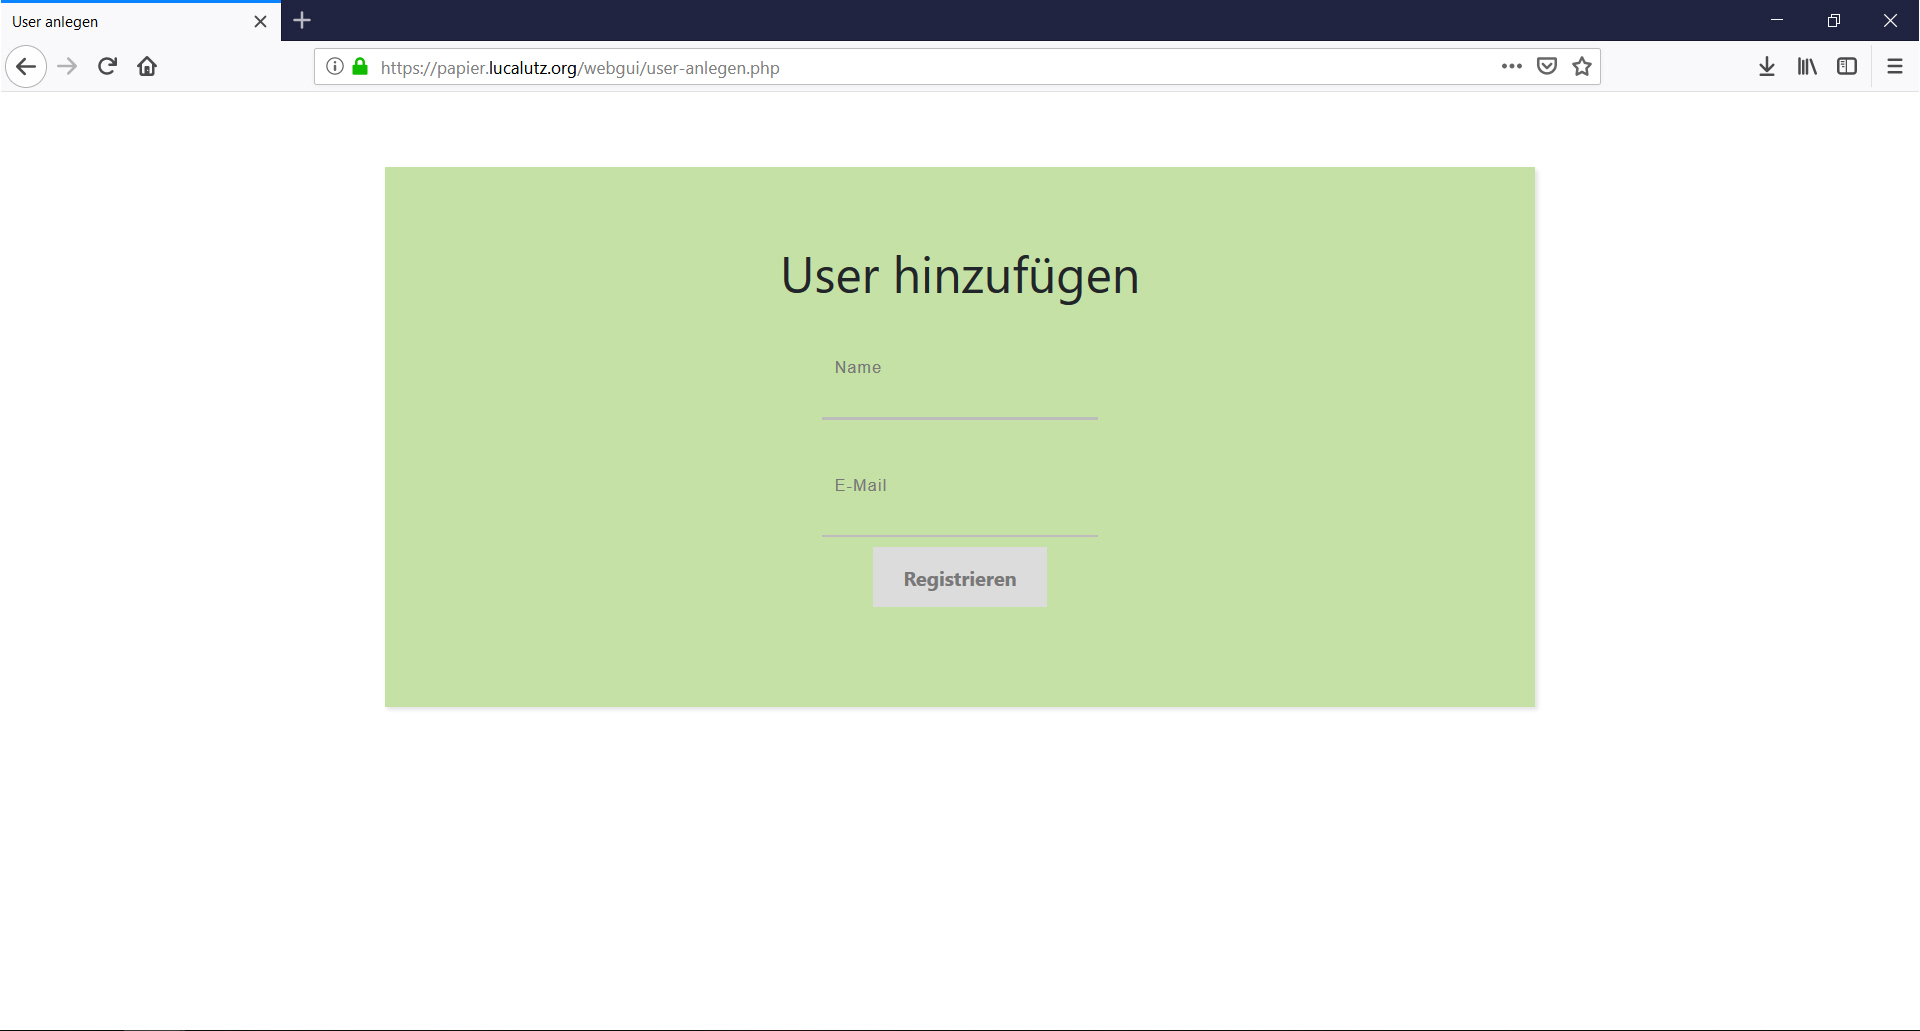
\includegraphics[width=0.7\textwidth]{user-anlegen.jpg} \\
    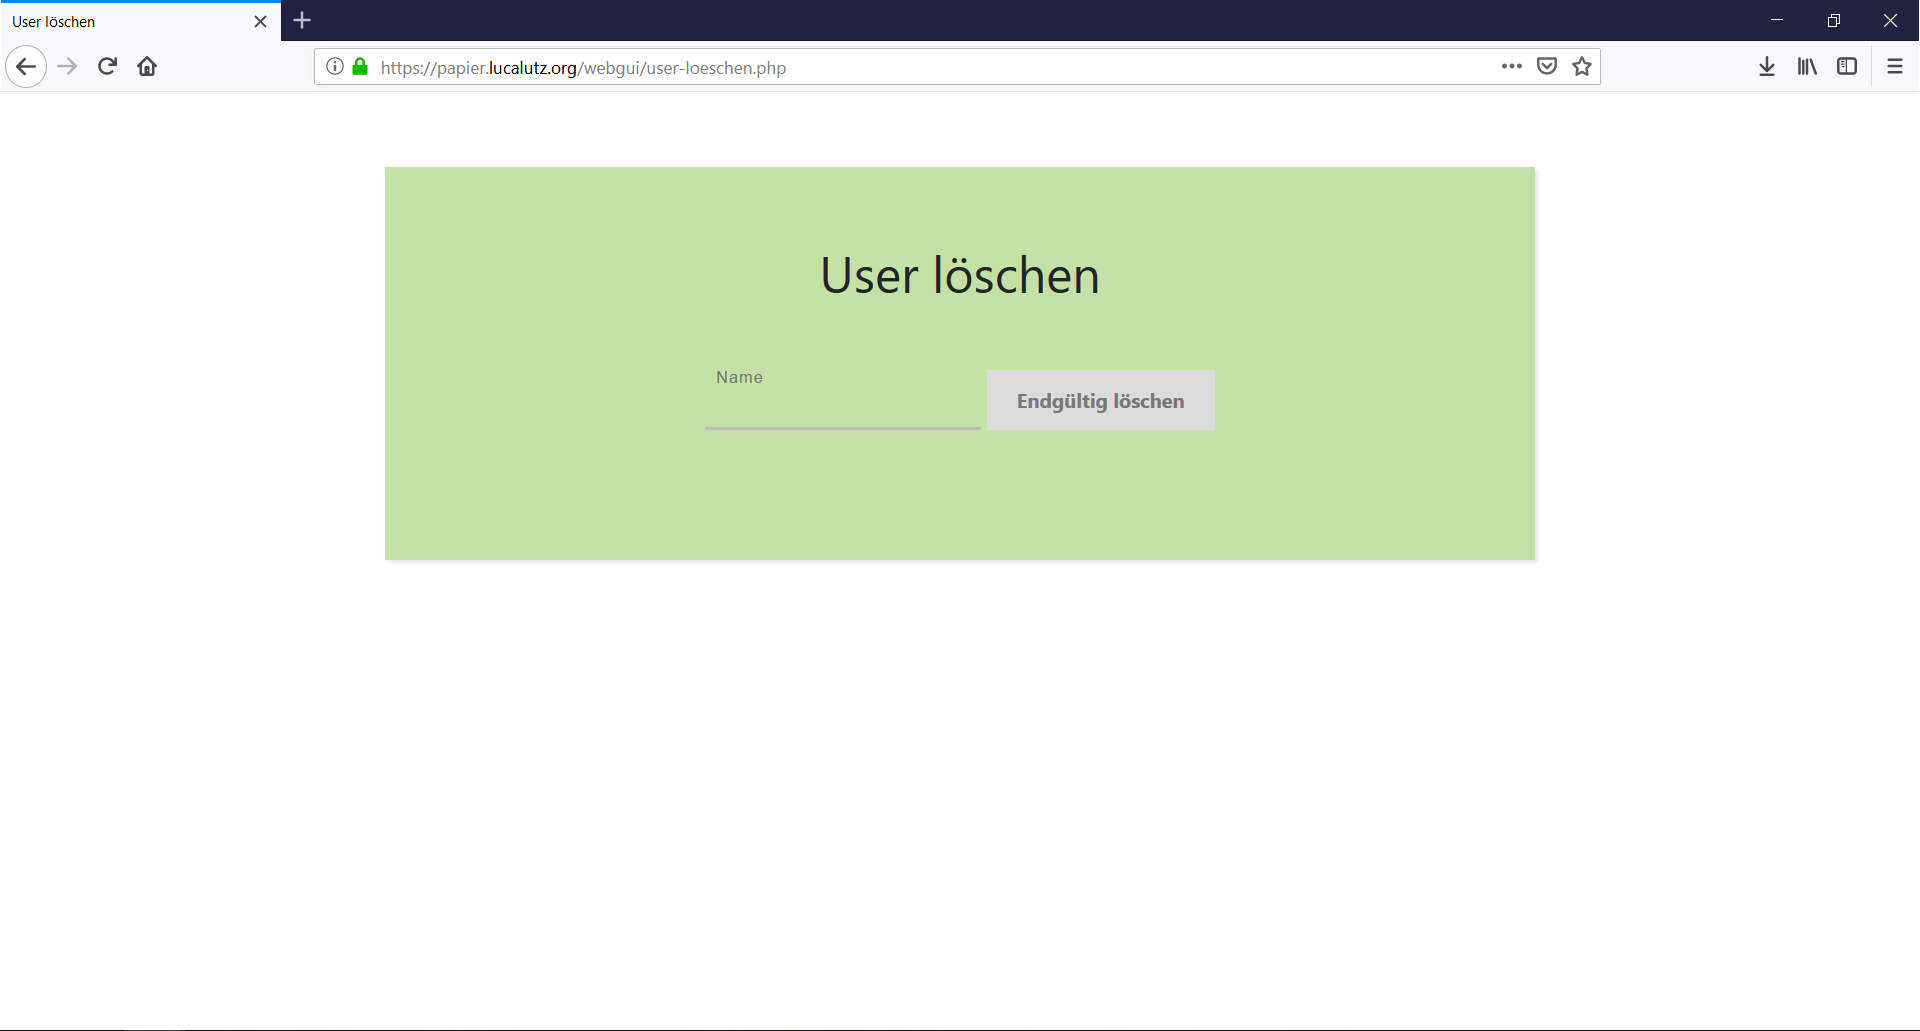
\includegraphics[width=0.7\textwidth]{user-loeschen.jpg} \\
    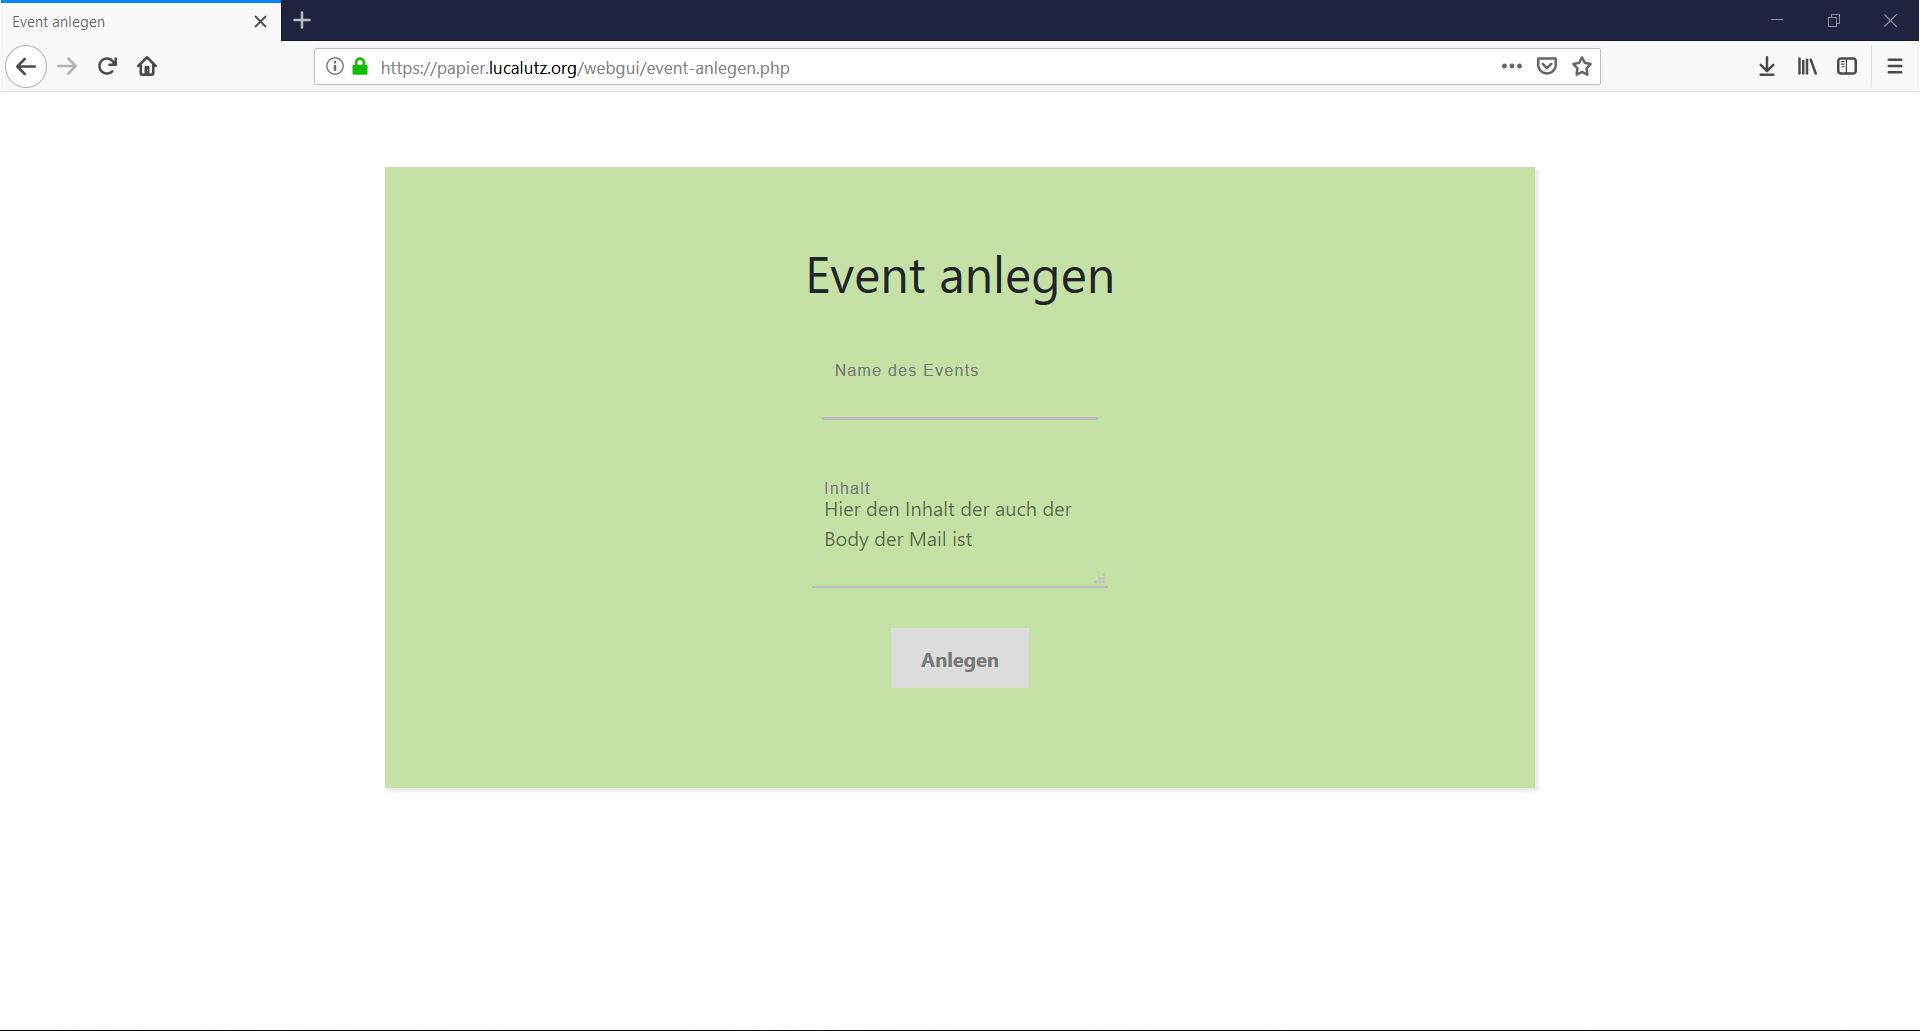
\includegraphics[width=0.7\textwidth]{event-anlegen.jpg} \\
    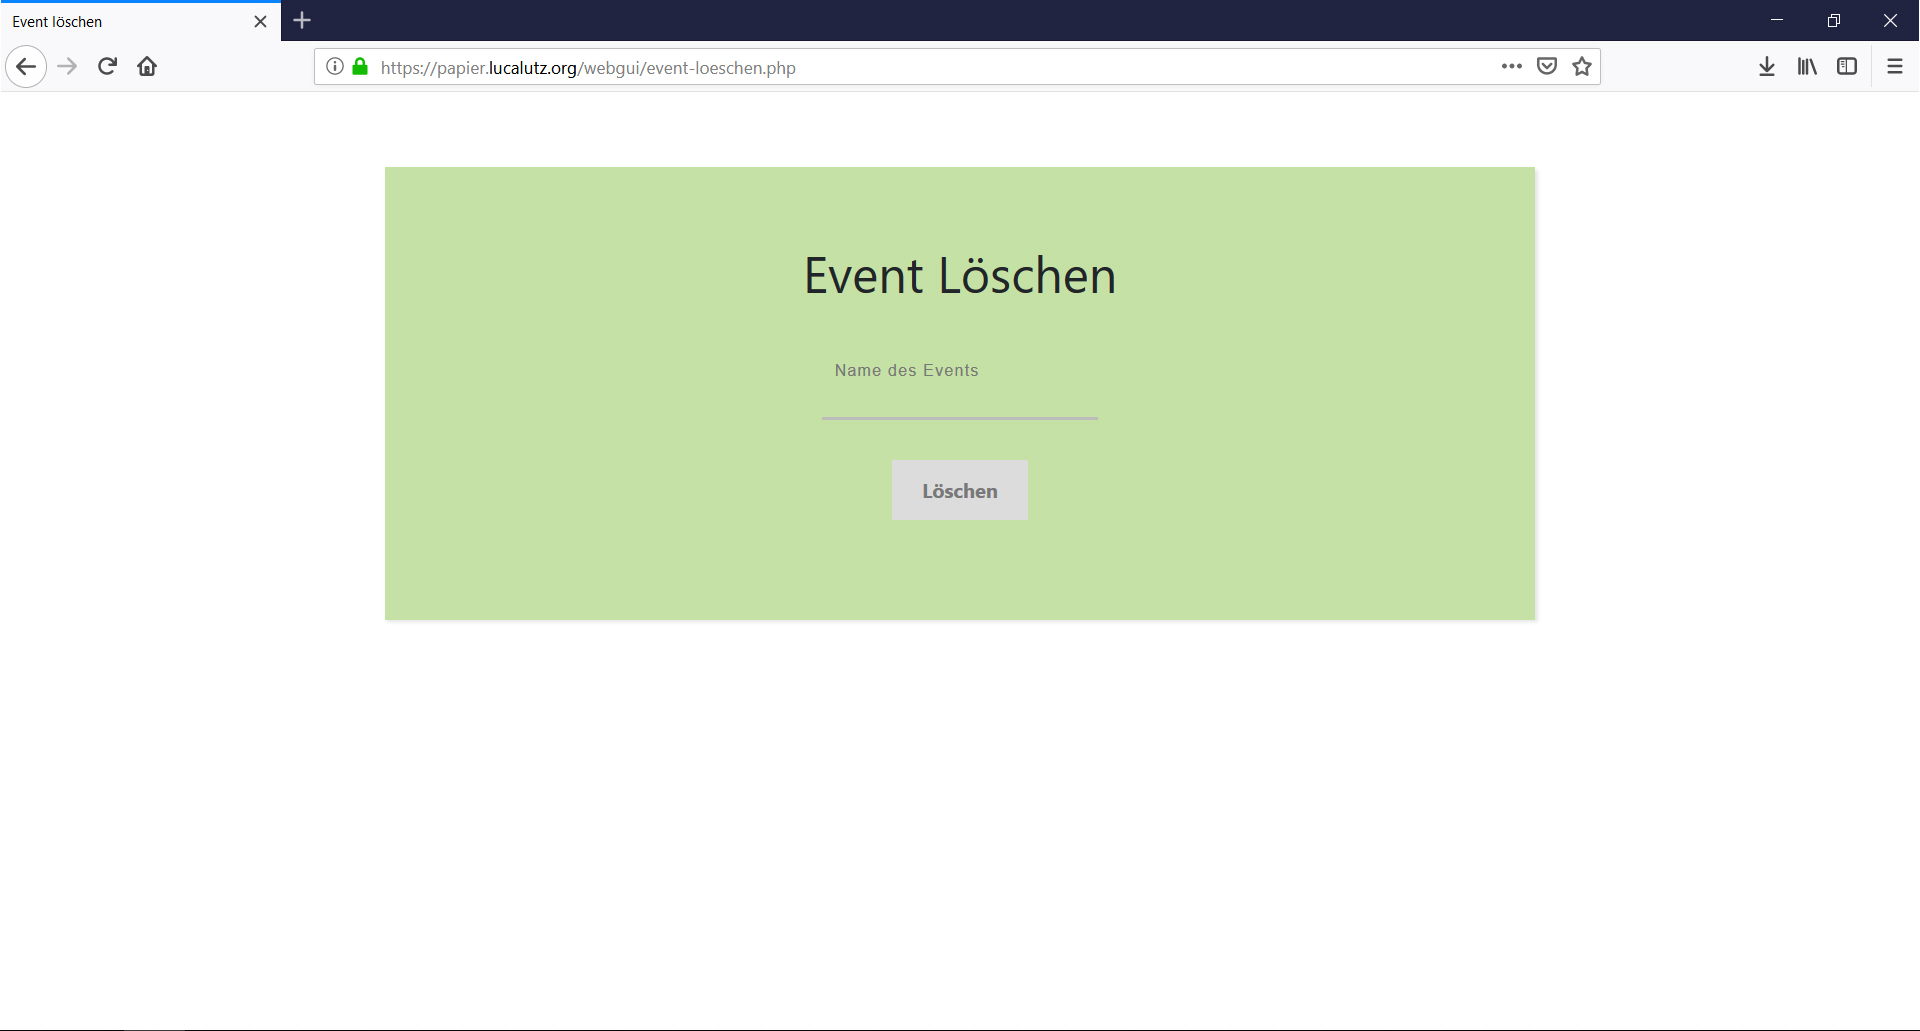
\includegraphics[width=0.7\textwidth]{event-loeschen.jpg} \\
  %\begin{figure}
   % \caption{Ein Event anlegen \label{EventAnlegen}}
  %\end{figure} 
  %\begin{figure}
  %  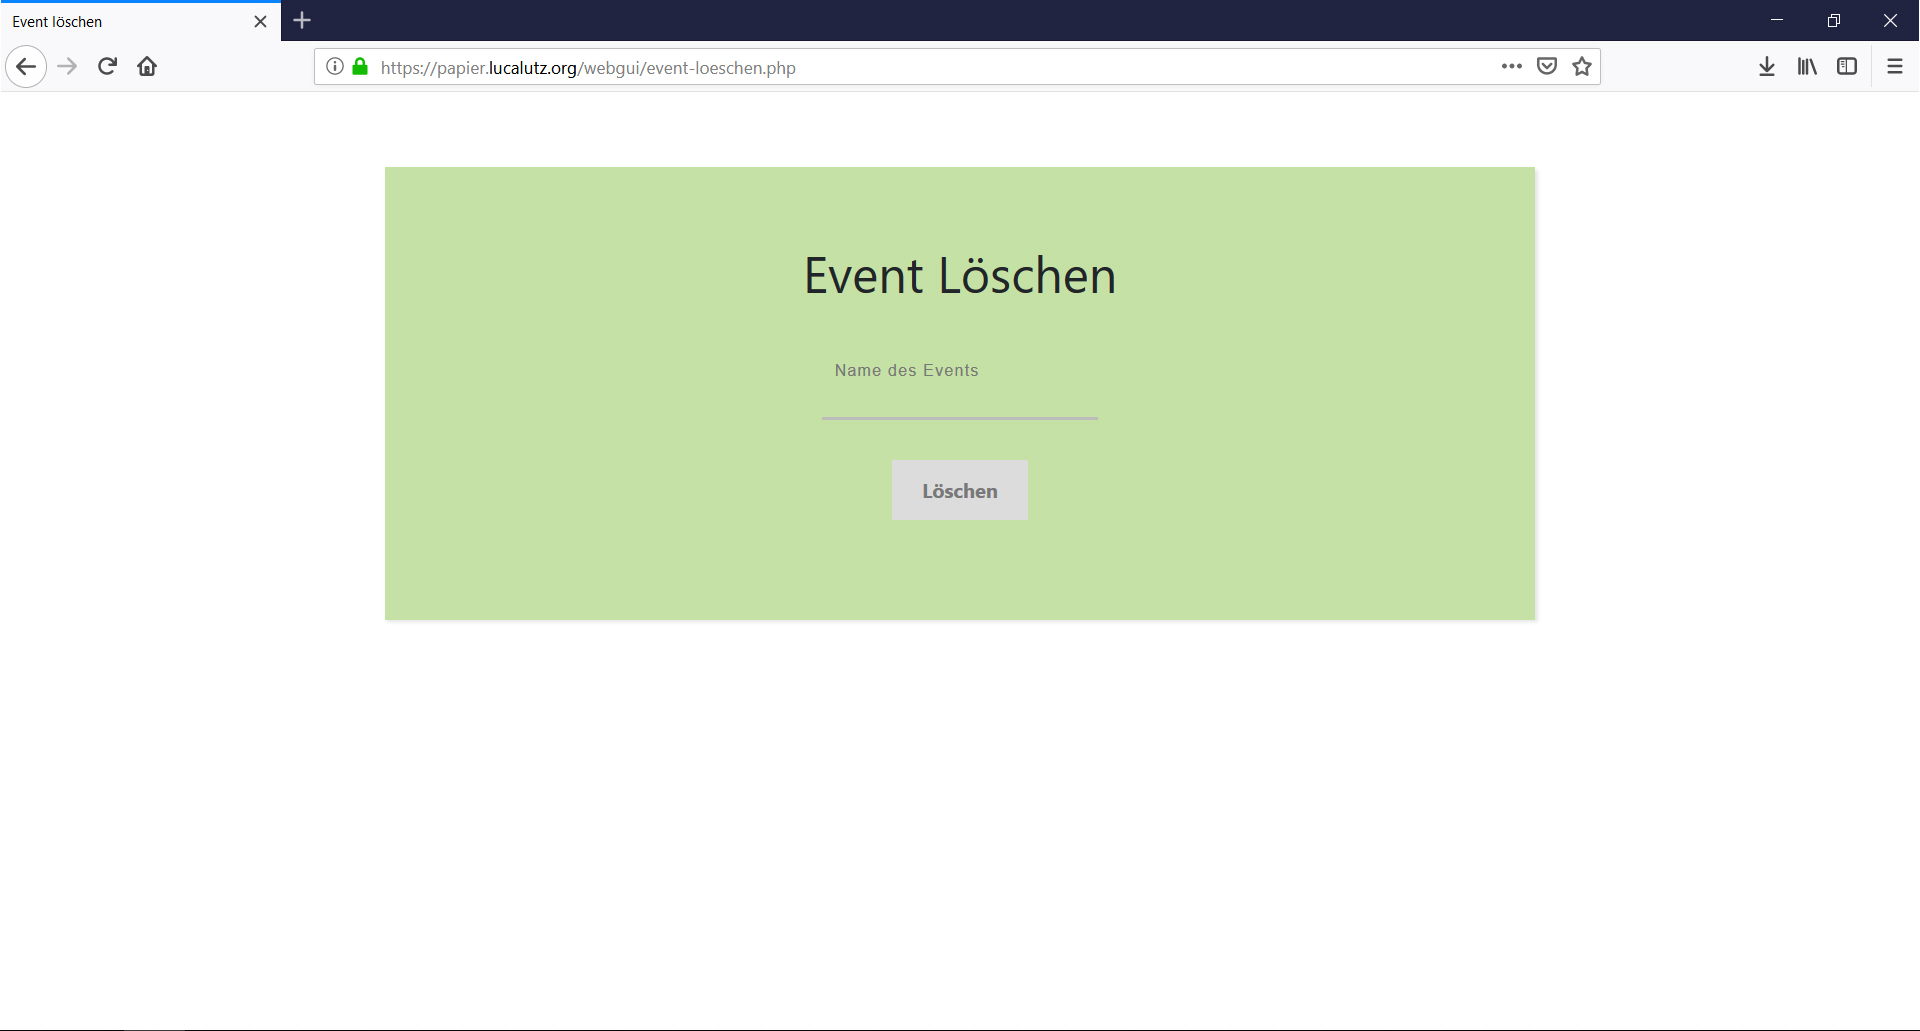
\includegraphics[width=0.7\textwidth]{event-loeschen.jpg}
  %  \caption{Ein Event l"oschen \label{EventLoeschen}}
  %\end{figure} 
  %\begin{figure}
    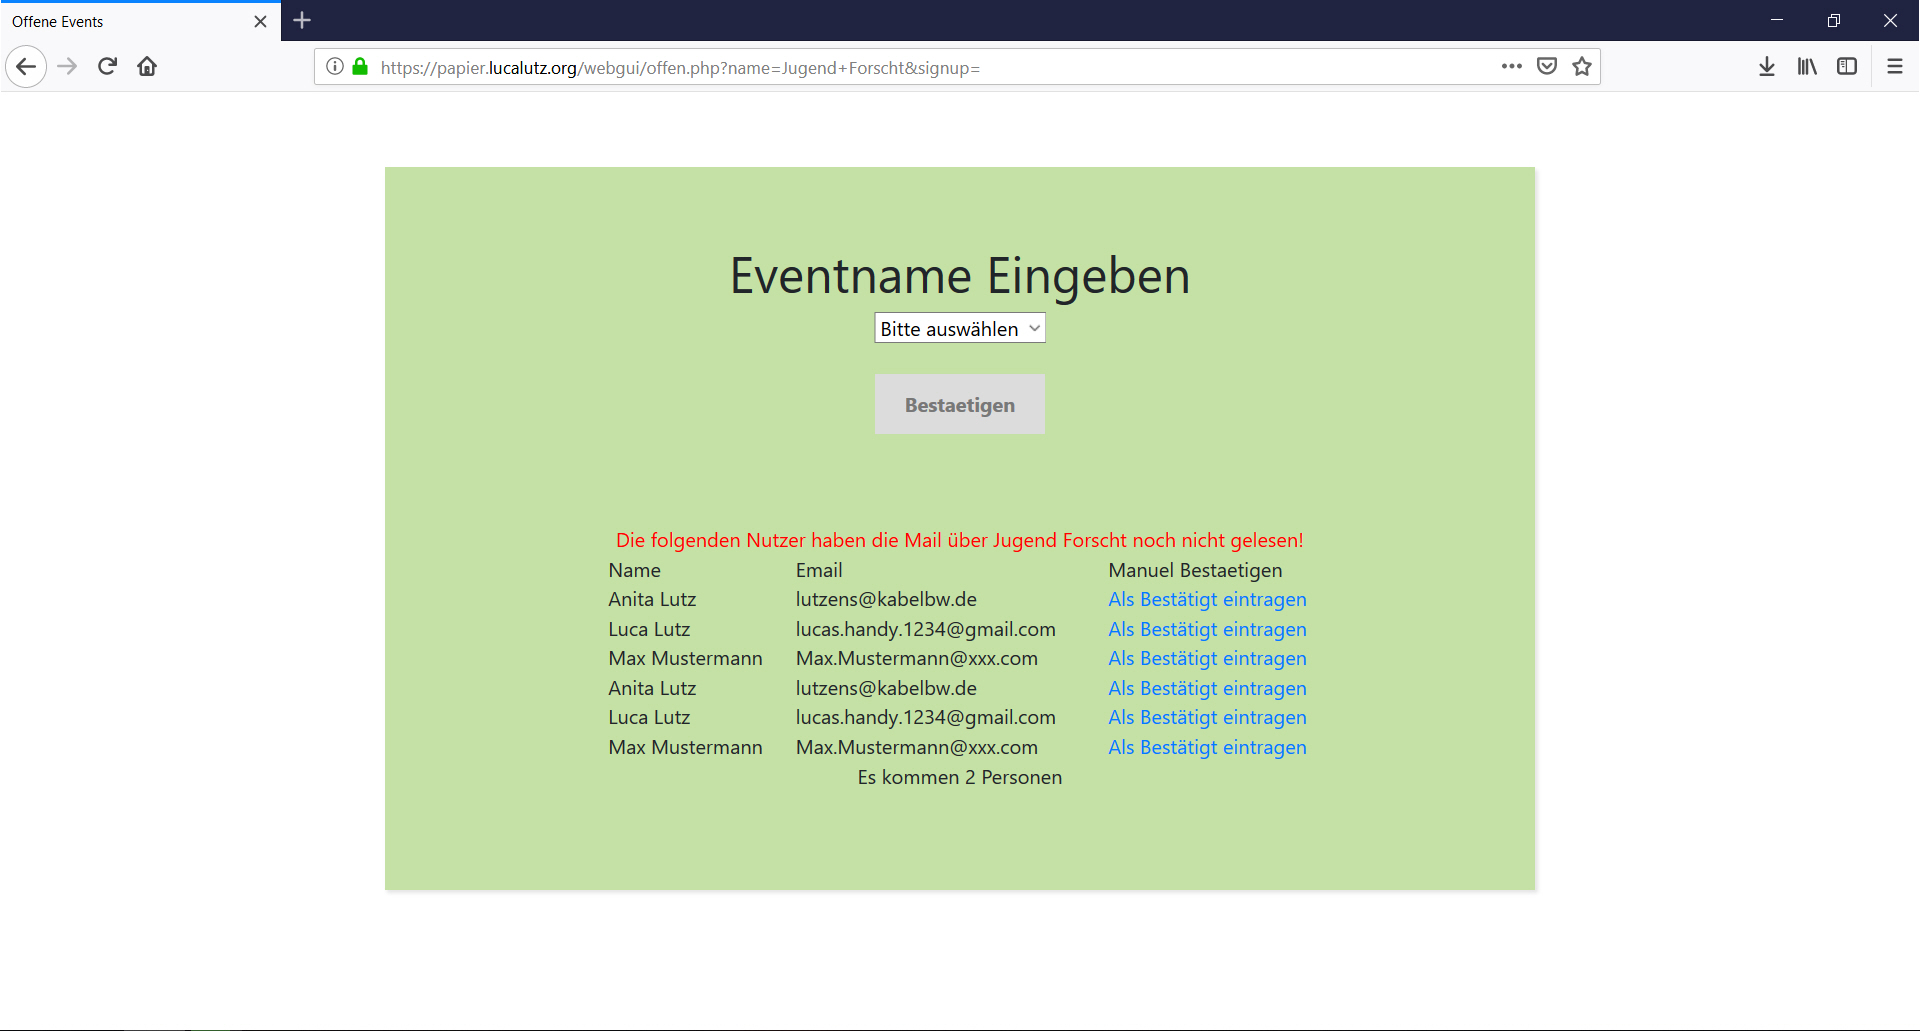
\includegraphics[width=0.7\textwidth]{offen.jpg} \\
  %  \caption{Offene Events ansehen \label{offen}}
  %\end{figure} 
  %\begin{figure}
    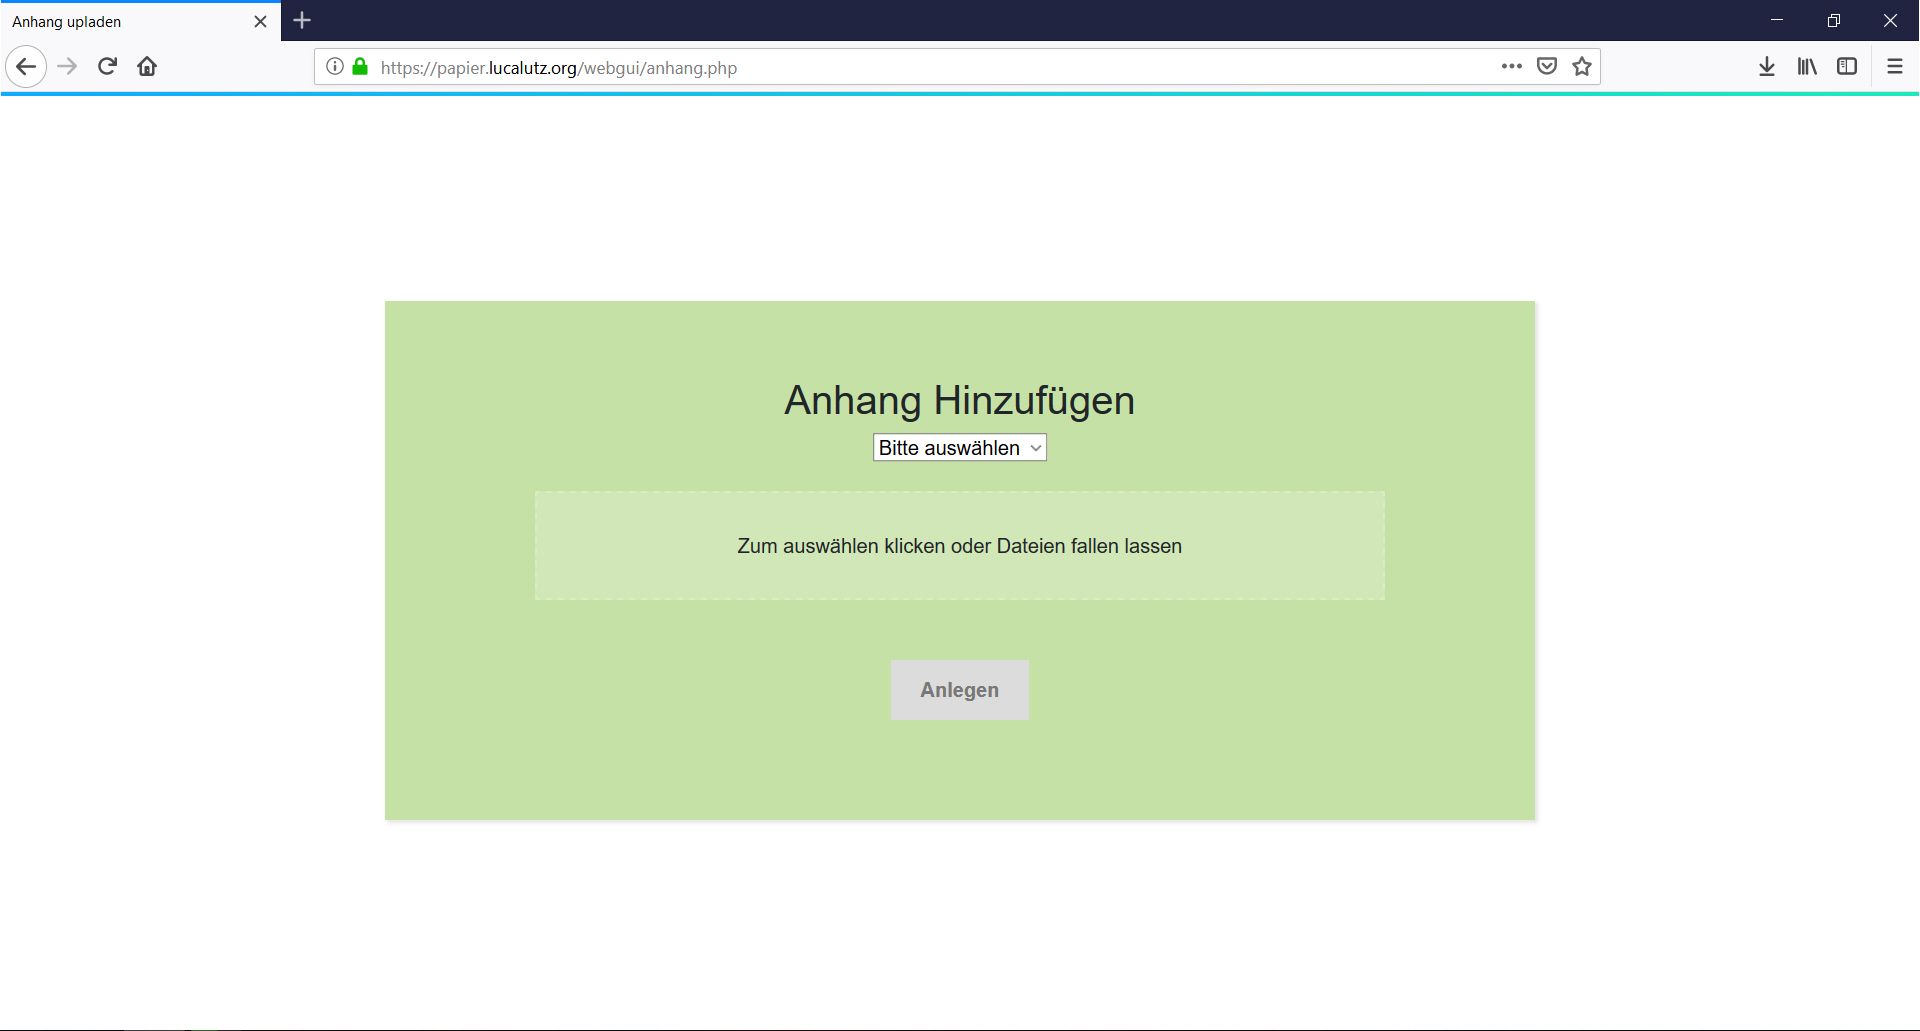
\includegraphics[width=0.7\textwidth]{anhang.jpg} \\
  %  \caption{Einen Anhang zu einem Event hinzuf"ugen \label{anhang}}
  %\end{figure} 
  %\begin{figure}
  %  \caption{Ein Mitglied anlegen \label{UserAnlegen}}
  %\end{figure} 
  %\begin{figure}
  %  \caption{Ein Mitglied l"oschen \label{UserLoeschen}}
  %\end{figure} 
  %\begin{figure}
    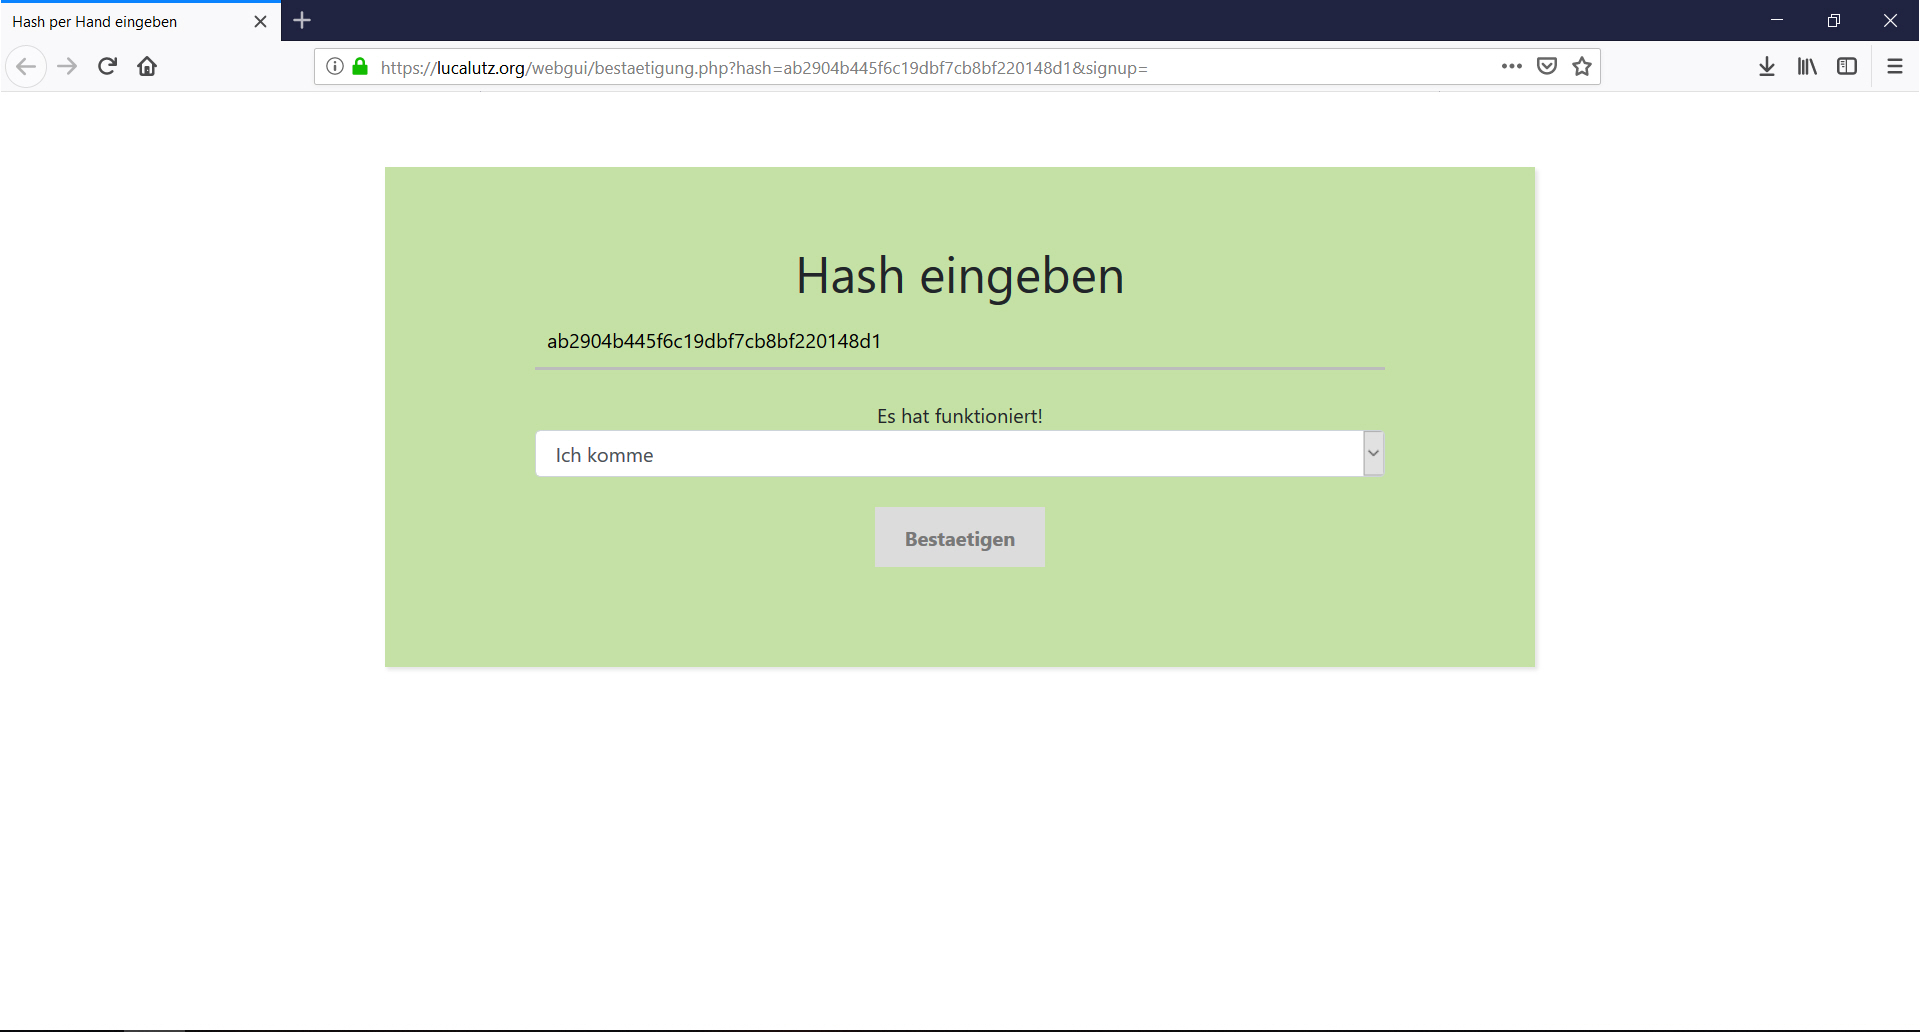
\includegraphics[width=0.7\textwidth]{bestaetigung.jpg} \\
  %  \caption{Die Eingabe zum best"atigen das Hashs \label{bestaetigung}}
  %\end{figure} 
  %\begin{figure}
  %  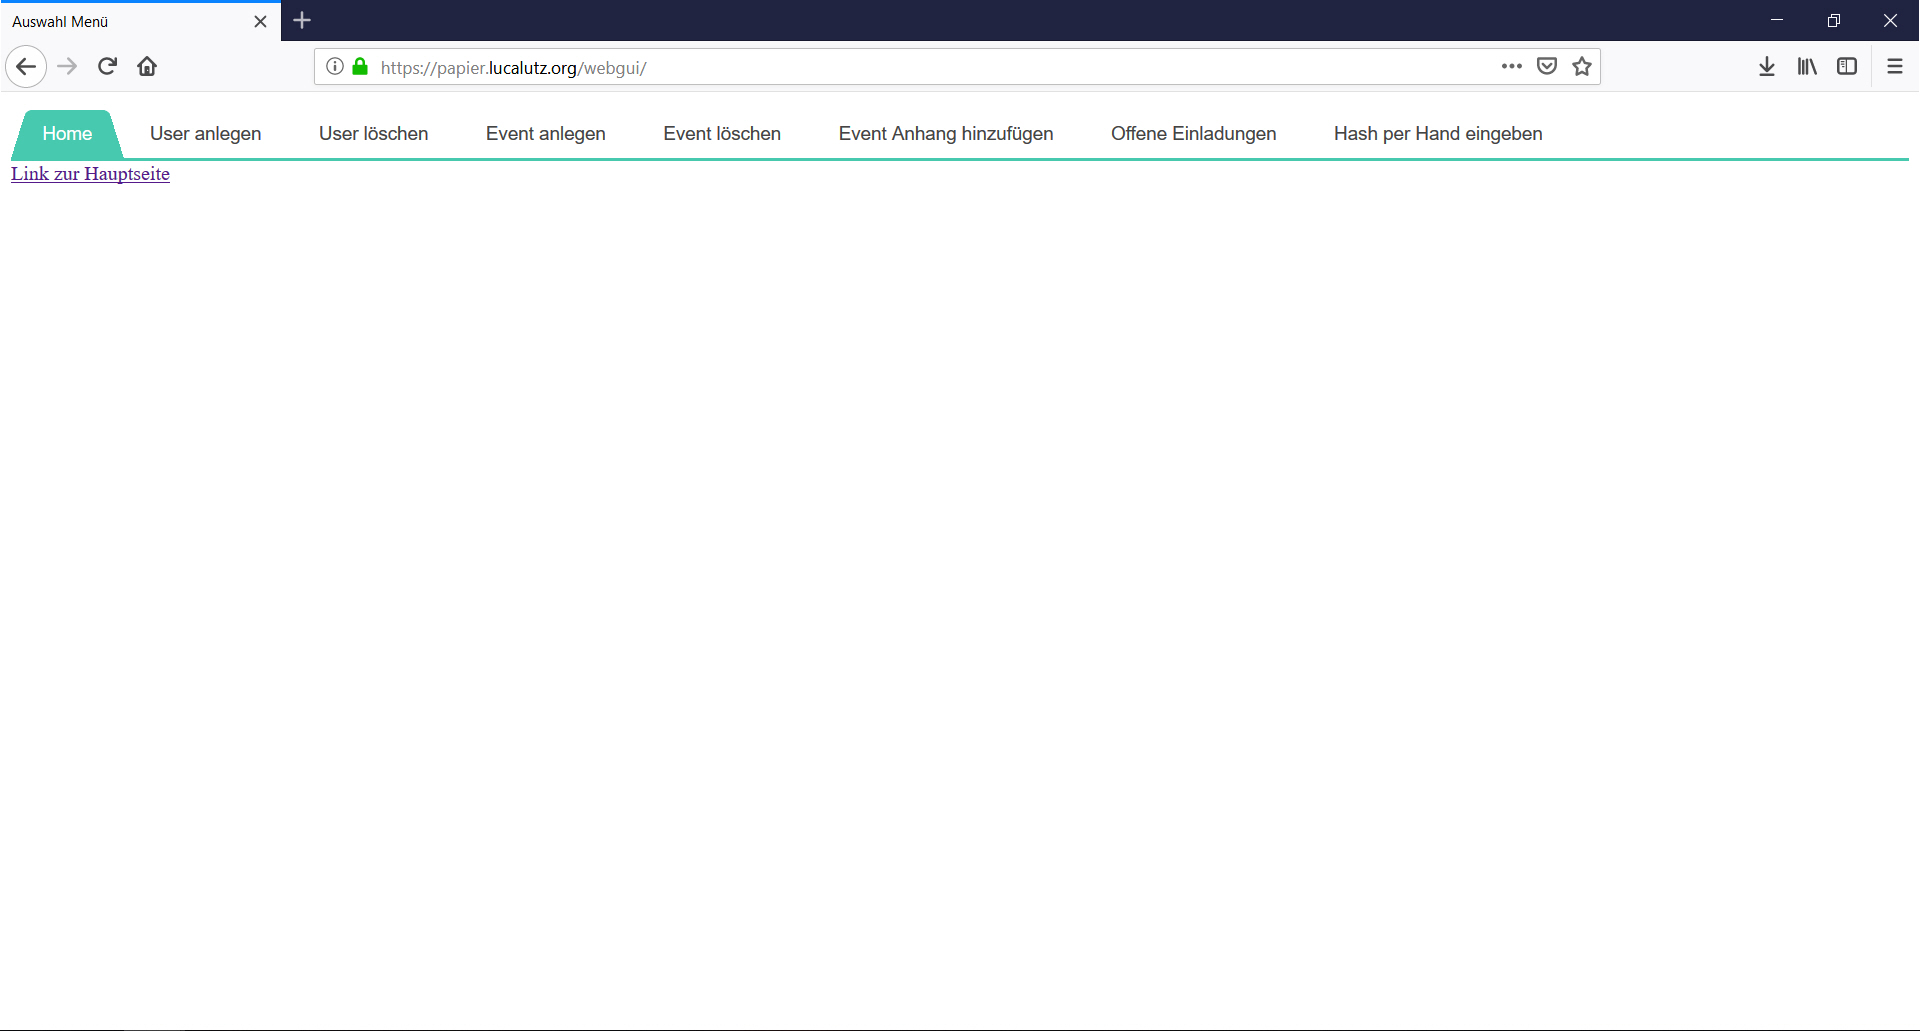
\includegraphics[width=0.7\textwidth]{index.jpg}
  %  \caption{Das Auswahlmen"u \label{auswahlmenue}}
  %\end{figure}  

    \section{Ergebnisdiskussion} % 1 Seite
    Meine Software kann nur Briefe im Plain-Text Format bearbeiten und nicht in 
    bin"aren Formaten wie z.B. PDF. Nat"urlich ist Plain-Text sehr beschr"ankt. So kann ich zum Beispiel 
    nichts unterstreichen oder Schriftarten setzen. Anstatt eine Plain-Text file will ich 
    f"ur die User ohne Internet und die die noch nicht geantwortet haben, ein PDF Dokument erzeugen.
    Eine weitere Idee w"are, dass ich auch Mails empfangen und somit 
    auch \glqq replays\grqq{} per Mail erm"oglichen kann.
    
    Herausforderung:
    Als Herausforderung hat sich vor allem die Aufgabe als vertrauensw"urdiger 
    Mailsender Mails zu versenden entpuppt, denn jede E-Mail, die ich sendete, landete 
    direkt im Spam Ordner. Dazu kam, dass ich anfangs nur per PHP in meine MySQL 
    Datenbank schreiben, aber nichts aus der Datenbank auslesen konnte.

  \section{Zusammenfassung} % 1/2 SeiteAnleitung 
  Mein Forschungsziel war es, Serienbriefe und Serienmails miteinander zu verbinden 
  und dadurch Papier zu sparen. Dieses Ziel habe ich in meiner Webgui und meinem Linux Postfix \cite{postfix} Script erreicht. 
  Es ist komplett mit der Kommandozeile "uber das Tool \glqq wget\grqq{} bedienbar.
  
  \textbf{Laut \cite{VereinsZahl} gibt es auf der ganzen Welt 15.644 Vereine. Mal angenommen 
  jeder davon h"atte 200 Mitglieder und jeder Verein versendet 2 Briefe auf Papier pro Jahr, dann 
  sind das 6.257.600 Blatt Papier f"ur Briefsendungen pro Jahr. Das sind 31,288 Tonnen
  unn"otig verbrauchtes Papier, plus weiteren 36,92 Tonnen Papier f"ur die Briefumschl"age. Hinzu 
  kommen 4.380.320,-\euro{} Versandkosten bei 70ct pro Briefporto. Allein die Kosten der Briefumschl"age betragen ca.: 360.000,-\euro{} \\ 
  Desweiteren muss ber"ucksichtigt werden, dass f"ur jeden dieser 
  Briefe eine gewisse Strecke mit den Verkehrsmitteln (Flugzeug bei weltweit aggierenden Vereinen; Auto...) anf"allt}.
  
  \section{Danksagung}
    Mein gr"o"ster Dank gilt Herrn Peter Wirsing, der Administrator und Betreuer im 
    SFZ Ulm ist und in Dornstadt wohnt. Besonders hat er mir bei der Informatik, 
    dem DNS, bei SSL, Linux, Mail, LaTeX, Dokumentation, Datenbank 
    und Organisation geholfen. Zudem unterst"utzt er mich bei dem selbst"andigen Suchen von Grammatik- und Zeichensetzungsfehlern. Daf"ur bin ich ihm sehr dankbar. \\
    Auch dem Vorstand der Concordia Westhausen, Herrn Hans Holl, gilt mein Dank, da er meine Software in der Praxis testet. \\
    Ebenso danke ich Christian Hendrich für seine Tipps und konstruktiven Anregungen. \\
    Zudem danke ich Letsencrypt f"ur die Ausstellung eines kostenlosen SSL Wildcard Zertifikats f"ur die Website und zum Mails versenden. \\
    Und nicht zu vergessen meiner Familie, die in der Zeit, in der ich mein Projekt umsetzte, mich nur zum Essen sah und gute Nerven mit mir nach einem schlechten Tag haben musste.

  \section{Ausblicke}
    Man k"onnte noch E-Post (vollautomatisches Versenden von Papierbriefen)in Betracht ziehen.
    Auch kann man die PHP zu Linux Br"ucke durch reines PHP ersetzen und die Anwendung somit auch z.B. unter einem Windows Webserver laufen lassen. 

  \section{Quellen}
  % \newpage \pagebreak % pw: wozu das denn?
  \begin{thebibliography}{15}
	\bibitem{php}         PHP,
			      Bitbucket Git system,
	                      \url{http://php.net/},
                              [Online; Stand 07.01.2019]
%	
	\bibitem{mysql}       MySQL,
			      MySQL SQL-system,
	                      \url{https://www.mysql.com/de/},
                              [Online; Stand 07.01.2019]
	
        \bibitem{LamaPool}    Lamapool Organisations Software,
			      Lapapool,
	                      \url{https://www.lamapoll.de/},
                              [Online; Stand 13.01.2019]
	
        \bibitem{softwareschichten} Softwareschichten,
			            Wikipedia,
	                            \url{https://de.wikipedia.org/wiki/Schichtenarchitektur},
                                    [Online; Stand 07.01.2019]
        
        \bibitem{Papiergewicht} Papier zu Tonnen,
                                Papiergewichtrechner,
			        \url{http://papiergewichtrechner.de/},
			        [Online; Stand 03.01.2019]

	\bibitem{git}         bitbucket,
			      Bitbucket Git system,
	                      \url{https://bitbucket.org},
                              [Online; Stand 03.01.2019]
	
	\bibitem{postfix}     Postfix,
			      Postfix Ratte,
	                      \url{https://de.postfix.org/},
       			      [Online; Stand 03.01.2019]

        \bibitem{AleitungLEC} Anleitung Lets Encrypt,
                              Luca Lutz,
			      \url{https://lucalutz.org/webgui/installation/wildcard_letsencrypt},
			      [Online; Stand 03.01.2019]
       
        \bibitem{VereinsZahl} Vereiszahlen,
			      Spiegel,
                              \url{https://magazin.spiegel.de/SP/2017/16/150556825/index.html},
			      [Online; Stand 03.01.2019]
	
        \bibitem{letsencrypt} Letsencrypt free Zertifikate,
		              Certbot inc.,
		              \url{https://letsencrypt.org},
			      [Online; Stand 03.01.2019]
	
	\bibitem{codetotex} PHP in Latex Code umwandeln,
		            Mark Liffiton,
		            \url{https://github.com/liffiton/code2tex},
			    [Online; Stand 03.01.2019]
	
	\bibitem{Doodle}    Doodle Organisator,
		            Doodle AG,
		            \url{https://doodle.com/de/online-umfrage-erstellen},
			    [Online; Stand 03.01.2019]

        \bibitem{Umrechner} Papier umrechner,
			    Papiernetz.de,
	                    \url{https://papiernetz.de/wp-content/uploads/Nachhaltigkeitsrechner_aktiv.pdf},
                            [Online; Stand 03.01.2019]

        \bibitem{Latex}     Latex Texteditor,
			    Latex
			    \url{https://www.latex-project.org/}
			    [Online; Stand 03.01.2019]

        \bibitem{Atom}      Atom Texteditor,
			    Mein HTML editor
			    \url{https://atom.io/}
			    [Online; Stand 03.01.2019]

        \bibitem{bootstrapExample} Bootstrap CSS example,
	                            Bootstrap,
			            \url{https://bootsnipp.com/snippets/or3WG},
				    [Online; Stand 03.01.2019]


	\bibitem{apache}    Apache2 Webserver,
			    Apache,
			    \url{https://httpd.apache.org/}
			    [Online; Stand 13.01.2019]
    \end{thebibliography}
\end{document}



